\section{Отслеживание контакта роликов при движении омни-колеса}\label{sect:track_omni}

% отсл конт
%     для (2) вообще надо пов-ти и град
%     омни
%         пов-ть
%         упс -- острие. плохо для град, но ок для сил 
%         ну таки возьмем да сложим вектора
%         усл (4) на углы и высоту
%         дифф вид для счета
%     меканум
%         обозн и что 4 поряд
%         неявн -- вектора
%         явн -- со ссылкой на СЯ
%     трение
%         вкл-выкл
%         выч норм (с пом (4)) и кас реакц
%         формулы для трения + про регуляриз по Нов

Чтобы получить явный вид уравнения\upr{eq:mo_cstr}, выражающего условие контактирования двух поверхностей, требуется найти радиусы-векто\-ры ближайших точек этих поверхностей и записать условия равенства проекций скоростей этих точек на общую нормаль поверхностей в этих точках.

Помимо этого, необходимо вычислить касательную составляющую скорости точки одного тела относительно другого для задания модели касательной составляющей реакции\upr{eq:mo_reac} в случае неидеальных связей.

% Для наглядности мы ограничиваемся рассмотрением омни-колес, оснащенных четырьмя роликами.  (Рис.~\ref{OmniWheel}).

% \begin{figure}[htb]
% \centering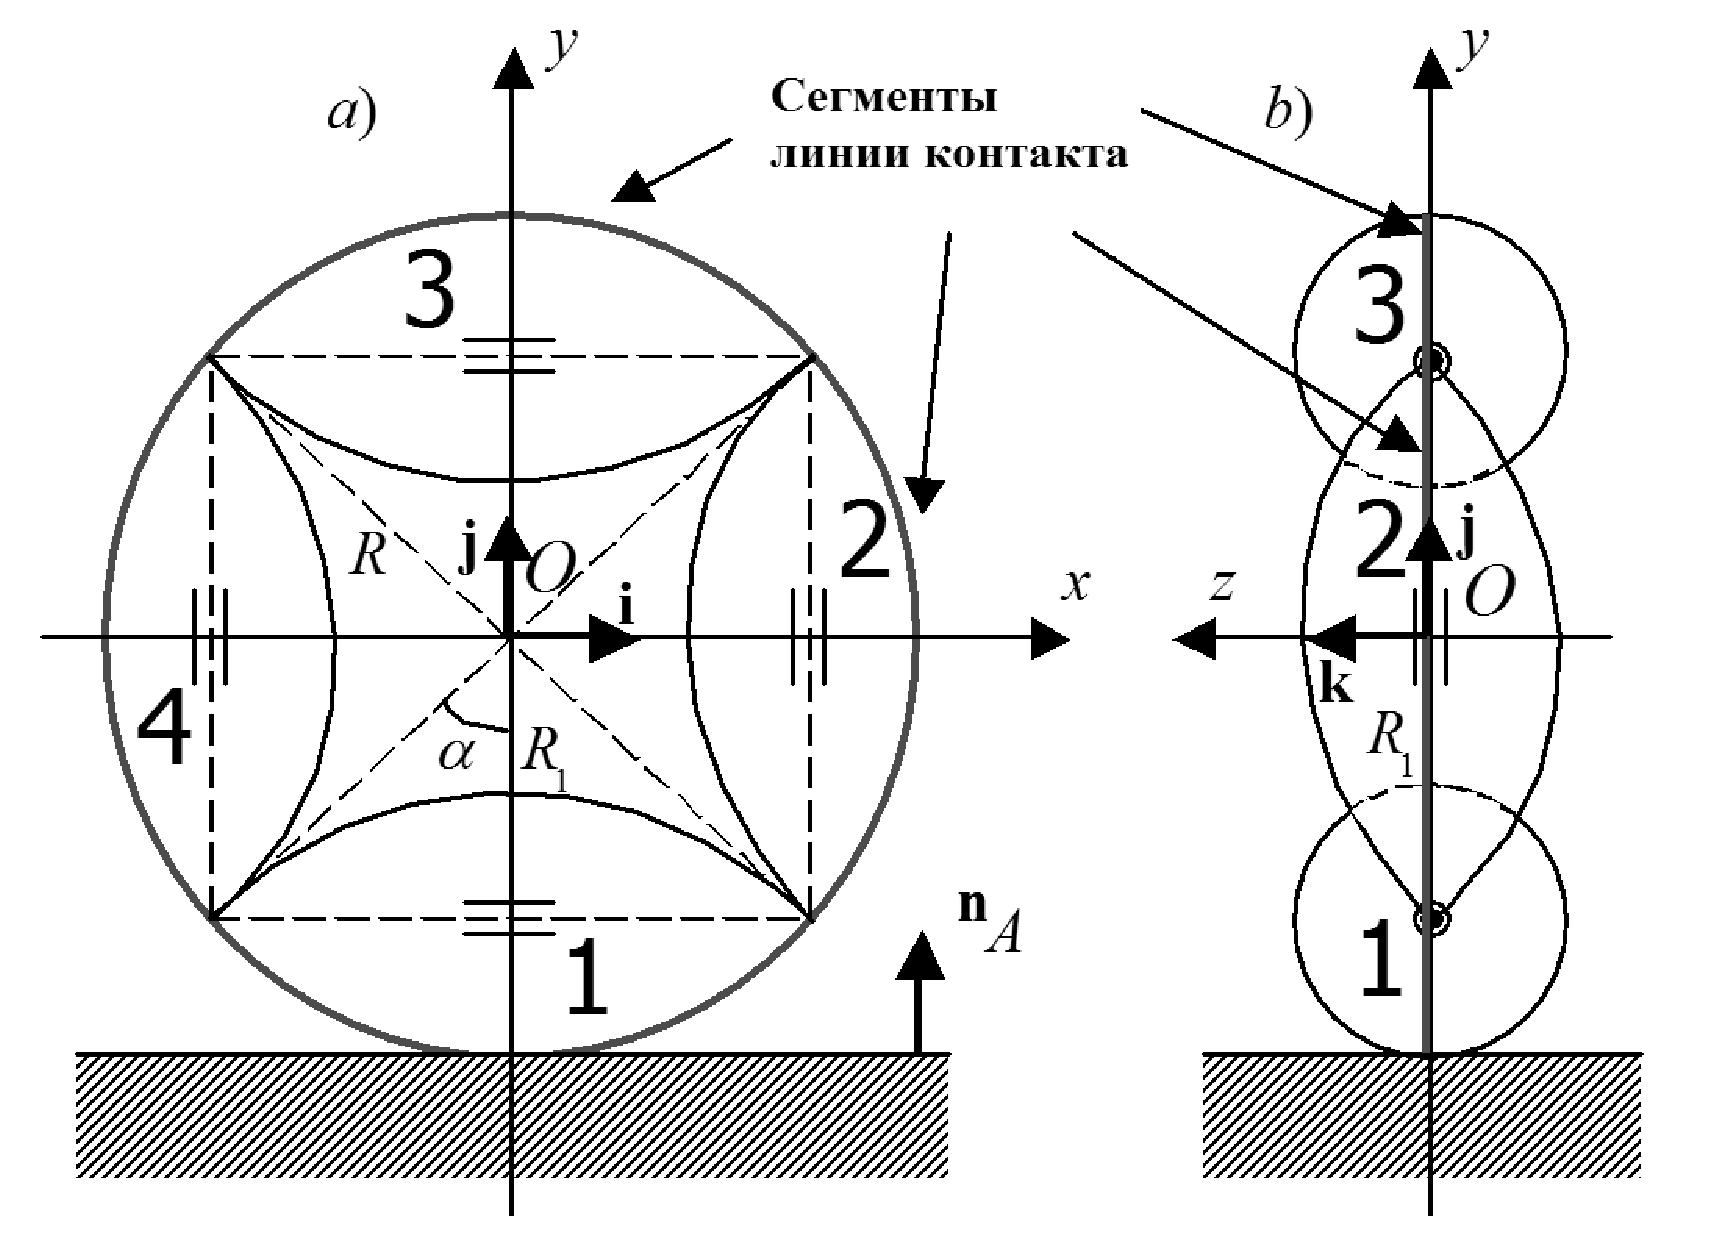
\includegraphics[width=13cm]{content/parts/3_friction/nd/OmniWheel.eps}
% \caption{Омни-колесо в вертикальном положении: a) вид сбоку; b) вид спереди.}
% \label{OmniWheel}
% \end{figure}


%Так что в результате переключение контактов между роликами омни-колеса не приведет к нарушению регулярности движения в силу причин ударного характера. Заметим еще раз, что все описанное будет справедливо, если колесо все время остается в вертикальном положении.

% На следующем уровне сборки модели несколько колес соединяются с подвижной 
% платформой экипажа при помощи шарнирных связей. В нашем случае количество колес 
% может быть три или более (в зависимости от конструкции экипажа и модели 
% контактирования ролика с полом). На платформе они могут образовывать самые 
% разные конфигурации. В конкретном примере Рис.~\ref{Vehicle} имеется три 
% колеса, образующие равносторонний треугольник в горизонтальной плоскости $zx$. 
% Ось $y$ здесь предполагается вертикальной.

% \begin{figure}[htb]
% \centering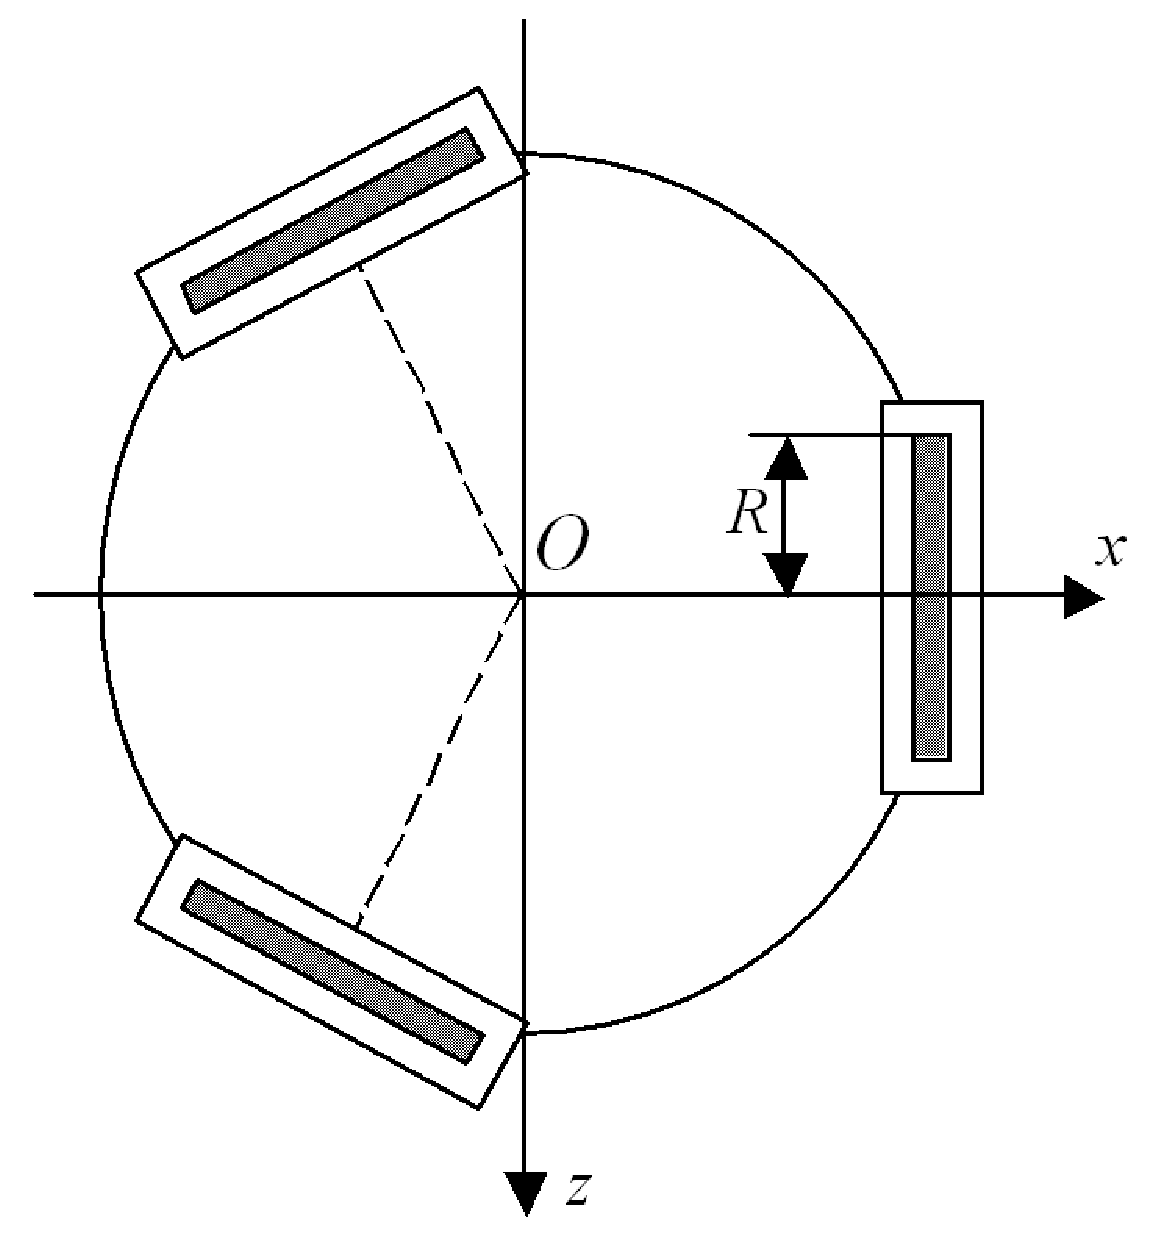
\includegraphics[width=9cm]{content/parts/3_friction/nd/Vehicle.eps}
% \caption{Трехколесный экипаж. Вид сверху.}
% \label{Vehicle}
% \end{figure}

% \section{Модель динамики отдельного ролика.\ }
% \label{sec3}

Для начала составим формулы, задающие геометрическую связь контакта между опорной плоскостью и одним неусеченным роликом колеса с $n$ роликами. Введем систему отсчета $Kxyz$, жестко связанную с роликом, следующим образом. Точку $K$ поместим в центр ролика, ось $x$ направим по продольной оси ролика, оси $y$ и $z$ расположим в плоскости, перпендикулярной оси $x$ и содержащей $K$. Напомним, что ролик ограничен поверхностью вращения дуги окружности радиуса $l$ вокруг ее хорды, отстоящей от центра $P$ на расстояние $r$ (обозначения см. на рис.~\ref{fig:wheel}), так что уравнение поверхности ролика в указанных осях имеет вид (см. фиг.~\ref{Roller}):
\begin{equation}
    x^2 + \left( \sqrt{ y^2 + z^2 } + r \right)^2 = l^2.
\end{equation}

\begin{figure}[htb]
    \centering
    % 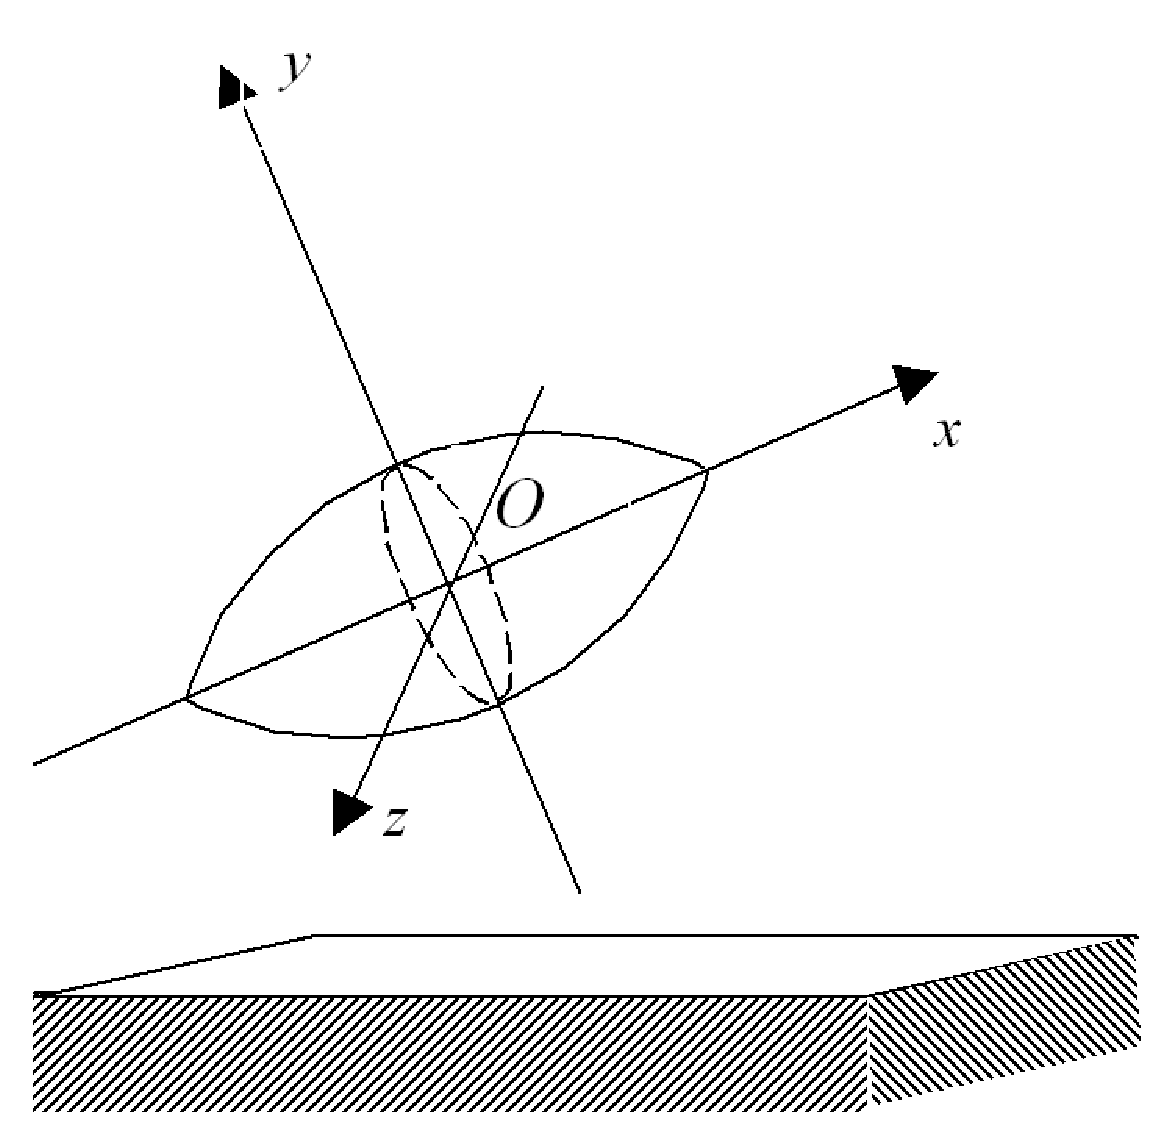
\includegraphics[width=10cm]{content/parts/3_friction/nd/Roller.eps}
    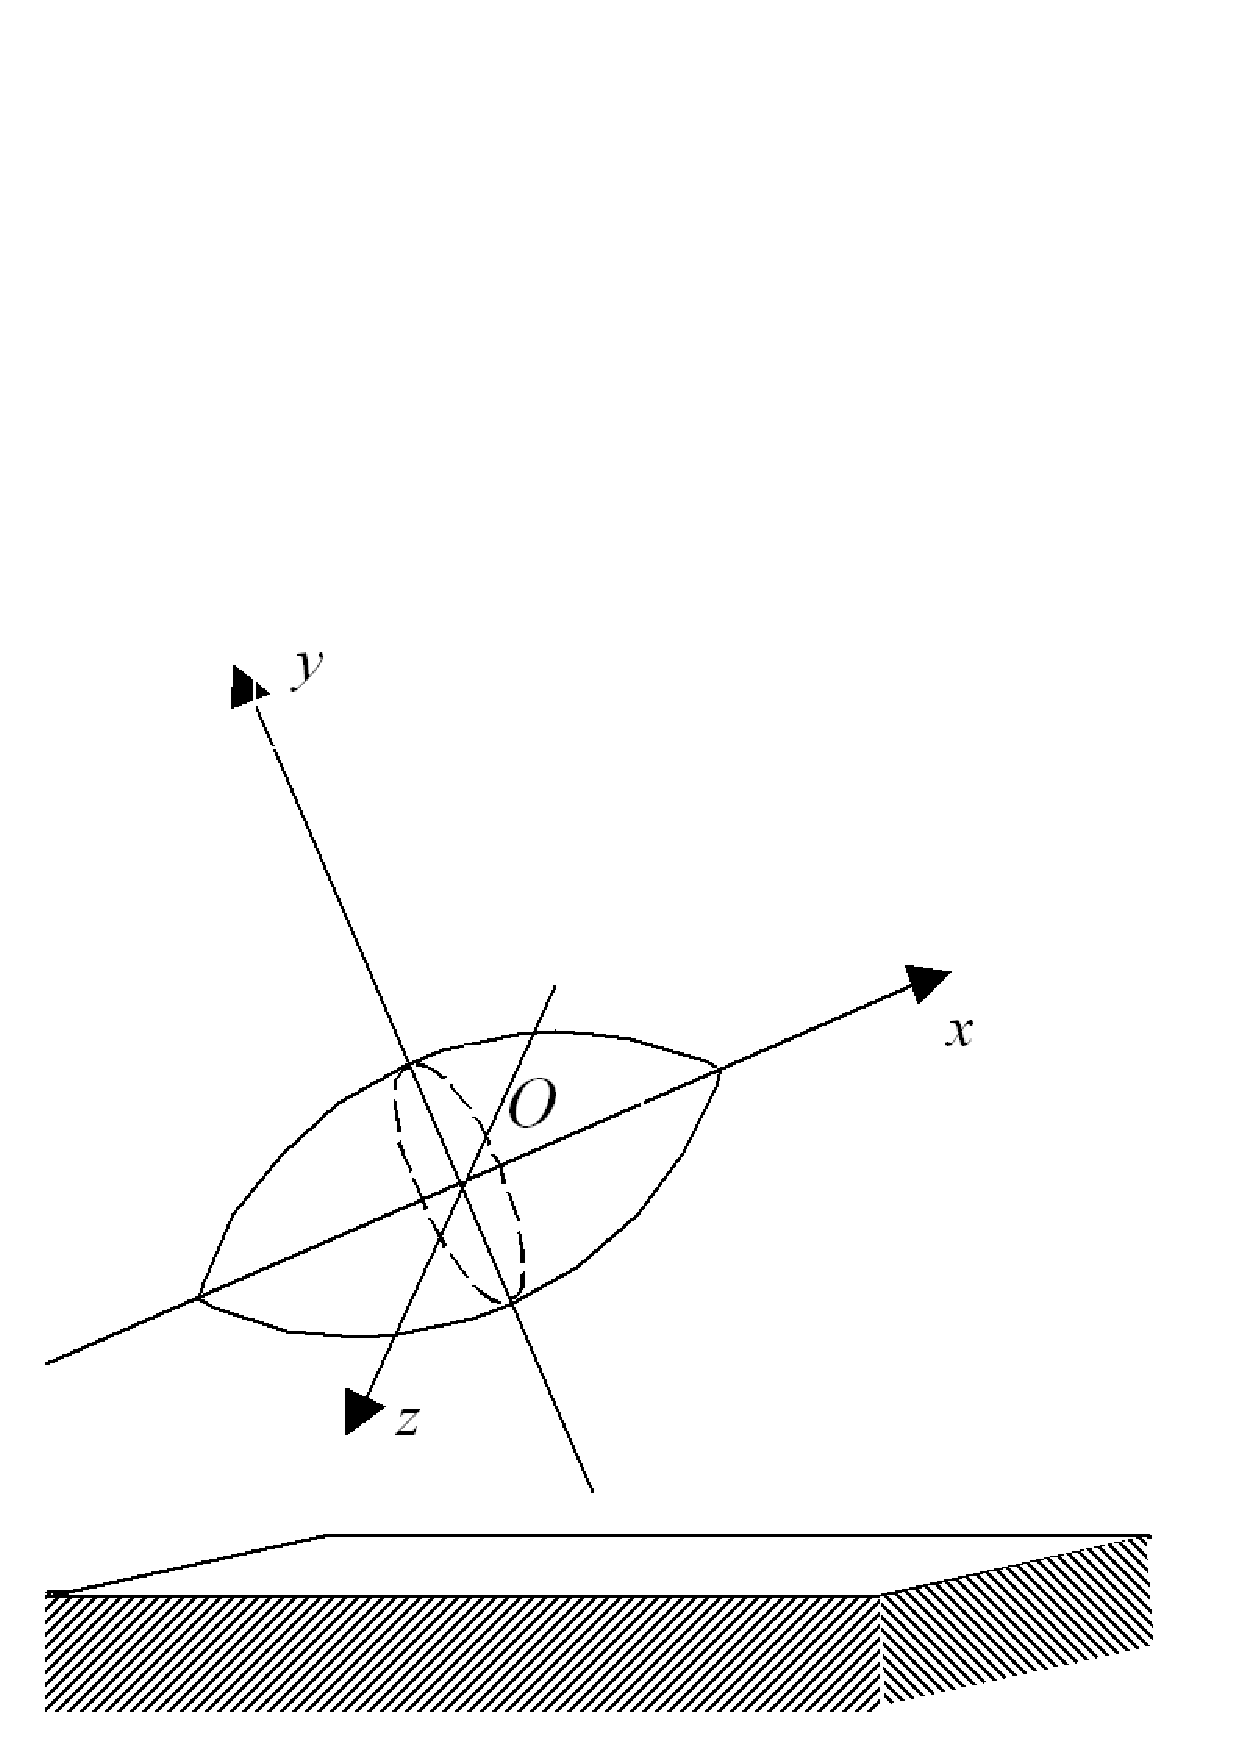
\includegraphics[width=10cm]{content/pic/modelica/Roller.png}
    \caption{Ролик над горизонтальной плоскостью.}
    \label{Roller}
\end{figure}

Заметим, что эта поверхность имеет  в 
точках $x=\pm \sqrt{l^2 - r^2}$ особенность, что в численных алгоритмах обычно приводит к аварийному завершению вычислительного процесса моделирования, так как требуется непрерывно вычислять градиент к поверхности ролика.

В задаче о движении экипажа с омни-колесами конфигурация системы твердых тел такова, что плоскости омни-колес остаются вертикальными во все время движения, и касательная плоскость к поверхности ролика определена при любом допустимом расположении тел. При этом условии можно указать явную формулу, позволяющую найти ближайшую к плоскости точку $C$ ролика: это вертикальная проекция центра колеса $P$ на плоскость.

\begin{figure}[htb]
    \centering
    % \includegraphics[width=8cm]{content/parts/3_friction/nd/RollerSection_d_ib.png}
    \asyinclude[width=12cm]{content/pic/asy/pic_roller_track.asy}
    \caption{Схема отслеживания контакта: вид сбоку отдельного ролика.}
    \label{ContactScheme}
\end{figure}

Найдем координаты точки $C$ (см. рис.~\ref{ContactScheme}). Обозначим $\vec{i}$ -- единичный направляющий вектор оси ролика, $\vec{r}_K$ -- радиус-вектор геометрического центра ролика в текущий момент времени и $\vec{\gamma}$ -- орт нормали к плоскости, в рассматриваемой задаче являющийся единичным вектором восходящей вертикали. Введем горизонтальный единичный вектор $\vec{d}$, перпендикулярный плоскости колеса следующим образом:
$$
    \vec{d} = \ddfrac
        {\vec{i} \times \vec{\gamma}}
        {\left| \vec{i} \times \vec{\gamma} \right|}.
$$
Пусть $P$ --- центр окружности, вращением дуги которой образована поверхность ролика (заметим, что эта же точка является центром омни-колеса). Тогда, очевидно, отрезок $\overrightarrow{KP}$, расположенный в вертикальной
плоскости, будет иметь длину $r$ и задаваться формулой
$$
    \overrightarrow{KP} = r\vec{d} \times \vec{i}.
$$
Так что радиус-вектор $\vec{r}_C$ самой нижней точки $C$ внешней поверхности ролика будет задаваться по формуле
\begin{equation}
    \vec{r}_C = \vec{r}_K + r\vec{d} \times \vec{i} - l\vec{\gamma},
\label{3_2_0}
\end{equation}
поскольку точка $K$ лежит на упоминавшейся выше окружности на общей вертикали с точкой $P$.

%Для вычисления положения точки $P_A$ нужно вторую координату 
%вектора ${\bf r}_{P_B}$ положить равной нулю
%\begin{equation}
%{\bf r}_{P_A}=\left( x_{P_B},0,z_{P_B}\right) ^T.
%\label{3_2_1}
%\end{equation}

Все описанные выше вычисления справедливы только, если вектор $\vec{i}$ имеет направление, составляющее с вертикалью $\vec{\gamma}$ угол, ограниченный значениями $\pm\left(\ddfrac{\pi}{2} - \ddfrac{\pi}{n}\right)$. В противном случае следует положить $C = B_\pm$, где $B_{-}$ и $B_{+}$ -- левая и правая концевые точки ролика соответственно (см. рис.~\ref{ContactScheme}).

Итак, условие контактирования ролика и плоскости можно записать в виде
\begin{equation}\label{cond:rol_vert}
    \left| \vec{i} \cdot \vec{\gamma} \right| \le \sin\ddfrac{\pi}{n}.
\end{equation}
Это условие, однако, позволяет из всего множества роликов колеса выделить два: нижний (контактирующий) и верхний. Чтобы отбросить последний случай, можно к полученному неравенству присоединить также требование 
\begin{equation}\label{cond:rol_low}
    Z_K < l
\end{equation}
где $Z_K$ -- расстояние от центра ролика до опорной плоскости.

Таким образом, конъюнкция условий (\ref{cond:rol_vert}) и (\ref{cond:rol_low}) означает наличие контакта. Реализация контакта геометрически означает выполнение скалярного условия
\begin{equation}\label{cond:rol_zero}
    Z_C = 0,
\end{equation}
позволяющего, вместе с уравнениями динамики твердого тела, вычислить величину нормальной реакции $F_n$, приложенной в точке $C$. Отсутствие контакта доставляет выполнение альтернативного, также скалярного, условия равенства нормальной реакции нулю
$$
    F_n = 0.
$$

Вычислительные эксперименты показали, что условие контакта в форме (\ref{cond:rol_zero}) обычно приводит к аварийному завершению процесса численного решения уравнений движения ролика. Аналогичный результат получается, если в качестве уравнения контактирования использовать уравнение, требующее равенства нулю нормальной составляющей скорости $v_n$ точки контакта: 
\begin{equation}\label{eq:cont_vn}
    v_n := \vec{v}_C \cdot \vec{\gamma} = \left(\vec{r}_C + \vec{\omega} \times \overrightarrow{KC}\right) \cdot \vec{\gamma} = 0.
\end{equation}
И только уравнение
\begin{equation}\label{eq:cont_Dvn}
    \dot{v}_n = 0
\end{equation}
приводит к требуемому результату -- корректной отработке процесса численного решения (выполняемого в данном случае инструментами языка \texttt{Modelica}~\cite{Fritzson}).

% Вся реализация процесса контактирования выполнена в предположении точечного <<твердого>> контакта твердых тел без какой-либо податливости.

% Колеса, собранные в экипаж, с неизбежностью будут сохранять вертикальное положение. Поэтому упрощенный алгоритм отслеживания контакта, описанный выше, всегда будет работать правильно.

Рассмотрение алгоритма отслеживания контакта в ролика омни-колеса и опорной плоскости завершено. В следующем разделе построим аналогичный алгоритм для ролика \textit{mecanum}-колеса, где ось ролика расположена под углом к плоскости колеса.